%%%%%%%%%%%%%%%%%%%%%%%%%%%%%%%%%%%%%%%%%
% Stylish Article
% LaTeX Template
% Version 2.1 (1/10/15)
%
% This template has been downloaded from:
% http://www.LaTeXTemplates.com
%
% Original author:
% Mathias Legrand (legrand.mathias@gmail.com) 
% With extensive modifications by:
% Israel Aguilera  (israel.aguilera.navarrete@gmail.com) Nov. 2022
%
% License:
% CC BY-NC-SA 3.0 (http://creativecommons.org/licenses/by-nc-sa/3.0/)
%
%%%%%%%%%%%%%%%%%%%%%%%%%%%%%%%%%%%%%%%%%

%----------------------------------------------------------------------------------------
%	PACKAGES AND OTHER DOCUMENT CONFIGURATIONS
%----------------------------------------------------------------------------------------

\documentclass[fleqn,10pt]{AmateCodex} % Document font size and equations flushed left

\usepackage[activeacute,spanish]{babel}

\fancyhead[R]{{\textsf{DOI-http}}\\
      {{\textsf{Agosto Diciembre, 2022. M\'{E}XICO}}}}
\fancyfoot[L]{{{Tlamatque \textbf{ISSN-xxx-xxx}}}}
\fancyfoot[C]{{{\textsf{P \'{a} g i n a \textbar  \textbf{\thepage} }}}}
\fancyfoot[R]{
\includegraphics[width=2.0cm]{imagenes/LOGO-Tlamatque2.pdf}}

%----------------------------------------------------------------------------------------
%	HYPERLINKS
%----------------------------------------------------------------------------------------

\usepackage{hyperref} % Required for hyperlinks
\hypersetup{hidelinks,colorlinks,breaklinks=true,urlcolor=blue,citecolor=blue,linkcolor=blue,bookmarksopen=false,pdftitle={Title},pdfauthor={Author}}

%----------------------------------------------------------------------------------------
%	ARTICLE INFORMATION
%----------------------------------------------------------------------------------------

\JournalInfo{Tlamatque, Vol. XXI, No. 1, 1-5, 2013} % Journal information
\Archive{DOI- htt} % Additional notes (e.g. copyright, DOI, review/research article)

\PaperTitle{Article Title} % Article title

\Authors{John Smith\textsuperscript{1}*, James Smith\textsuperscript{2}} % Authors
\affiliation{\textsuperscript{1}\textit{Department of Biology, University of Examples, London, United Kingdom}} % Author affiliation
\affiliation{\textsuperscript{2}\textit{Department of Chemistry, University of Examples, London, United Kingdom}} % Author affiliation
\affiliation{*\textbf{Corresponding author}: john@smith.com} % Corresponding author

\date{Recibido: \today / Aceptado: 18 marzo 2023}

\Keywords{Keyword1 --- Keyword2 --- Keyword3} % Keywords - if you don't want any simply remove all the text between the curly brackets
\newcommand{\keywordname}{Keywords} % Defines the keywords heading name

%----------------------------------------------------------------------------------------
%	ABSTRACT
%----------------------------------------------------------------------------------------
\Abstract{El resumen es la síntesis de lo que aparecerá en el artículo. 
Tiene que ser lo suficientemente consiso para que alguien sepa qué esperar del artículo si lo leyera completo. 
Puede concluir con palabras clave. 
El resumen queda fuera de la numeración del resto de secciones.
Es una descripción abreviada de la investigación, sin la interpretación del autor, contiene toda la información que incluye el informe final, haciendo hincapié en sus puntos sobresalientes.}
%----------------------------------------------------------------------------------------

\begin{document}

\flushbottom % Makes all text pages the same height
\maketitle % Print the title and abstract box
\tableofcontents % Print the contents section
\thispagestyle{empty} % Removes page numbering from the first page


%----------------------------------------------------------------------------------------
%	ARTICLE CONTENTS
%----------------------------------------------------------------------------------------

\section{Introduction} % The \section*{} command stops section numbering

En la introducción se deben especificar aspectos, cuyo significado depende del tipo concreto de artículo:

\begin{enumerate}[noitemsep]
\item Planteamiento del problema
\item Definición del problema
\item Delimitación del problema
\item Hipótesis
\item Justificación
\item Marco teórico
\end{enumerate}

Una buena introducción debe lograr que el lector tenga interés de leer el resto del artículo.

\subsection{Planteamiento del problema}

Es la descripción sistemática y rigurosa de los hechos y acontecimientos que giran en torno a una determinada situación donde se mencionan algunos antecedentes, se precisa qué aspectos se van a estudiar de un determinado fenómeno, hecho o problema, enfatizando las características que más interesa investigar.


\subsection{Definición del problema}

Es la especificación de la problemática existente sobre el tema, al nivel que se esté trabajando: institucional, local, estatal, regional o nacional.

\begin{enumerate}[noitemsep]
 \item Identificar todos los problemas, describiéndolos someramente y tratando de darles una posible explicación.
 \item Determinar cuál es el problema más importante: planteándolo, delimitándolo y definiéndolo.
 \item Formularlo de manera inteligible y precisa, claramente y sin ambigüedades, evitando las palabras confusas.
 \item Buscar problemas similares resueltos, revisando literatura sobre el problema o cuestiones afines para utilizar soluciones y procedimientos para su solución.
 \item Proponer diversas explicaciones (hipótesis) de las causas del problema.
 \item Encontrar, entre las explicaciones, aquellas que permitan adquirir una visión más profunda de la solución del problema.
 \item Hallar relaciones entre los hechos y las explicaciones.
 \item Determinar cuáles son los elementos principales del problema, reduciéndolo a sus aspectos esenciales, variables o dimensiones.
 \item Plantear una pregunta que exprese una relación entre dos o más variables; esto al final de una descripción que se haga de la problemática.
 \item Se puede descomponer la pregunta original en varias interrogantes secundarias.
\end{enumerate}

\subsection{Delimitación del problema}

Es la forma de acotar el problema, ubicándolo dentro de un contexto geográfico o temporal.

\begin{enumerate}[noitemsep]
 \item Geográficas o espaciales: señalando la región geográfica donde se realizará la investigación (región, zona, territorio, institución, etc.).
 \item Temporales: señalar si la investigación se llevará a cabo en un período determinado (estudio transversal) o en el transcurso del tiempo (estudio longitudinal).
\end{enumerate}

Situar el problema en el contexto geográfico o temporal.


\subsection{Hipótesis}

Proposición, suposición, supuesto, predicción, conjetura o explicación tentativa susceptible de ser probada que postula una relación causal entre dos o más variables identificadas, basada en los conocimientos ya existentes, o bien en hechos, fenómenos y relaciones nuevas y en el marco teórico organizado y sistemático que se ha estructurado previamente, por lo que es la mejor explicación al problema en cuestión. Esto hace avanzar el conocimiento científico, porque aceptando o rechazando hipótesis se confirman o modifican las teorías; permite aislar lo esencial, lo significativo; contribuye a descubrir la naturaleza del fenómeno; sirve para delimitar y especificar más el o los problemas; sirve para generalizar y ampliar los conocimientos; sugiere explicaciones; orienta la investigación; dirige la búsqueda del orden entre los hechos; ofrece posibilidades de proporcionar una respuesta adecuada a los problemas planteados; introduce coordinación en el análisis y orienta la elección de los datos; establece los límites del estudio. Esta orientación o idea directriz que guía la investigación debe ser abandonada, mantenida o rectificad, una vez obtenidos los resultados. Si es apoyada por los datos empíricos, ha sido confirmada y pasa a formar parte de la teoría científica; cuando no corresponde con los datos empíricos, ha sido refutada. Sin embargo, aún aquellas hipótesis que resultan falsas tienen valor, ya que al ser rechazadas hacen avanzar el conocimiento, pues se descarta y reduce el número de posibilidades entre las cuales debe buscarse la relación objetiva.

Las clasificaciones son de carácter convencional. Sirven para distinguir propósitos, funciones, niveles, o procedimientos. Algunas formas de clasificación son las siguientes:

\begin{enumerate}[noitemsep]
 \item Por el número de variables: las que involucran una variable y las que involucran dos o más.
    \begin{enumerate}
      \item Las que involucran una sola variable: \textquotedblleft Los investigadores educativos son, por lo general, apolíticos \textquotedblright.
      \item Las que relacionan dos o más variables: \textquotedblleft A mayor nivel de escolaridad de los investigadores educativos, mayor nivel de ingresos \textquotedblright.
    \end{enumerate}
 
\item Por la forma de relación entre variables:

\begin{enumerate} [noitemsep]
 \item Oposición $(+ \ldots -)$  $(- \ldots +)$    A mayor $ \ldots $ menor $ \ldots $ ;   A menor $ \ldots $ mayor $ \ldots $
 \item Paralelismo $(+ \ldots +)$   $(- \ldots -)$   A mayor $ \ldots $ mayor;    A menor $ \ldots $ menor $ \ldots $
 \item Causa-efecto  $(x \ldots y)$  Si $ \ldots $ entonces $ \ldots $ (ejemplo.  \textquotedblleft Si existieran las condiciones adecuadas en las instituciones, entonces sería posible un mejor desarrollo de la investigación en México \textquotedblright).
\end{enumerate}

\end{enumerate}

\subsubsection{Elementos de la hipótesis}

\begin{enumerate}[noitemsep]
 \item Las unidades de análisis (individuos, grupos, vivienda, etc.).
 \item Las variables, o sea, las características o propiedades cualitativas o cuantitativas que presentan las unidades de análisis.
 \item Los elementos lógicos que relacionan las unidades de análisis con las variables o éstas entre sí.
\end{enumerate}


\subsubsection{Sugerencias}

\begin{enumerate}[noitemsep]
 \item Dar respuesta al problema o problemas propuestos.
 \item Enunciarlas de tal modo que por medio de las técnicas de investigación aceptadas puedan ser probadas.
 \item Prever técnicas para probarlas.
 \item Clasificarlas, jerarquizarlas y ordenarlas.
 \item Mantener las hipótesis hasta haber obtenido resultados.
\end{enumerate}

\subsection{Justificación}

Tiene como finalidad dejar en claro por qué es importante realizar el estudio.

\subsubsection{Sugerencias}
Puede elaborarse planteando lo siguiente:

\begin{enumerate}[noitemsep]
 \item Beneficios que se obtendrán al resolver algunos de los problemas planteados, aclarando qué se resolverá.
 \item Alcances y aplicación: años y áreas en que podrán aplicarse los resultados.
 \item Impulso a otras investigaciones.
 \item Contribuciones o solución a un problema.
 \item Aportaciones a la teoría.
 \item Productos de la investigación (parciales, laterales y finales): proyectos, informes, programas, manuales, apuntes, artículos, libros, ponencias, conferencias, propuestas didácticas, tesis, etc.
 \item Población que se beneficiará con los resultados: alumnos, profesores, academia, institución, el mismo investigador, etc.
\end{enumerate}

\subsection{Marco teórico}
Es la inserción del problema en un determinado cuerpo de conocimientos científicos, manejando críticamente lo que ya se conoce sobre el tema en lo referente a teorías y a resultados de investigaciones realizadas en el propio campo de interés. Se establece a través de una revisión bibliográfica exhaustiva, pero limitada a los temas que tienen relación con el problema planteado.


\subsubsection{Sugerencias}

\begin{enumerate}[noitemsep]
 \item Revisar objetivos, metodología y conclusiones de investigaciones recientes y de parecida índole. Hacerlo cronológicamente (ascendente o descendente).
 \item Describir la relación del problema con investigaciones anteriormente realizadas.
 \item Revisar teorías que expliquen el enfoque de la investigación (educativas, filosóficas, psicológicas, económicas, sociológicas, etc.).
\end{enumerate}

\cite{Figueredo:2009dg}, \cite{Morgan}

%------------------------------------------------
\section{Materiales y métodos}
La palabra método se deriva de las raíces griegas metá y odos (Metá – movimiento; odos – camino). Etimológicamente quiere decir “camino hacia algo”; camino a seguir mediante una serie de operaciones y reglas fijadas de antemano, de manera voluntaria y reflexiva, para alcanzar un cierto fin. Por lo tanto, es el camino producto de la experiencia acumulada, racionalizada y probada en el desarrollo histórico de la ciencia que conduce al conocimiento, el cual no es inmutable y es imposible tenerlo proyectado en todos sus detalles; dicho camino se va haciendo o, al menos, se va completando como resultado de la actividad científica. Es el procedimiento lógico, esbozo, esquema, proceso, prototipo o modelo que indica las operaciones intelectuales, las decisiones, pasos, fases etapas o actividades que han de llevarse a cabo para realizar una investigación en una situación esperada o prevista con lo cual se pueden combinar resultados relevantes con economía de procedimientos. Con ello de pretende controlar las situaciones con las que se enfrenta la investigación, incluyendo lo referente a tipo de investigación, procedimiento para desarrollarla, fuentes de información, características de la población, muestreo empleado, descripción de instrumentos empleados, modalidades de acopio y registro de datos; forma en que se procesó y analizó la información y la manera en que se presentan los resultados. Además, pueden incluirse los recursos financieros y materiales disponibles, así como el equipo humano que realizará la investigación. Por su parte, la palabra metodología se deriva de las raíces griegas metá, odos y logos, donde éste último término significa tratado. Entonces, etimológicamente metodología quiere decir estudio o tratado del método.

\paragraph{Sugerencias}

\begin{enumerate}[noitemsep]
 \item Plantear los métodos ya probados, aunque no se pretenda utilizarlos exactamente de la misma manera y, muchas veces, se les introduzcan algunas modificaciones.
 \item Incluir lo referente a tipo de investigación, procedimiento para desarrollarla, procedimiento para recopilar y analizar la información así como para la presentación de resultados.
\end{enumerate}


\begin{table}[t]
\caption{Technical solutions of a bicycle front wheel.}  
\begin{center}
\label{TSwell}
  \begin{tabular}{lp{6cm}}
\hline\noalign{\smallskip}
Item & Technical solution\\
\noalign{\smallskip}\hline\noalign{\smallskip}
$ts_1$ & Fast assembly connection 133mm (5-1/4") \\
$ts_2$ & Axis and hub 108mm (4-1/4")\\
$ts_3$ & Locknut 3mm\\
$ts_4$ & Flat washer 1.5mm\\
$ts_5$ & Cone (M9x12.8mm) with dust cover and seal ring\\
$ts_6$ & Seal ring\\
$ts_7$ & Axis 108mm (4-1/4")\\
$ts_8$ & Balls (3/16") 20 items\\
$ts_9$ & Rim\\
$ts_{10}$ & Beam 278mm\\
$ts_{11}$ & Nipple\\
$ts_{12}$ & Tag A\\
$ts_{13}$ & Tag C\\
$ts_{14}$ & Tire\\
$ts_{15}$ & Tube\\
\noalign{\smallskip}\hline
\end{tabular}
    \end{center}
\end{table}

\begin{figure*}[ht]\centering % Using \begin{figure*} makes the figure take up the entire width of the page
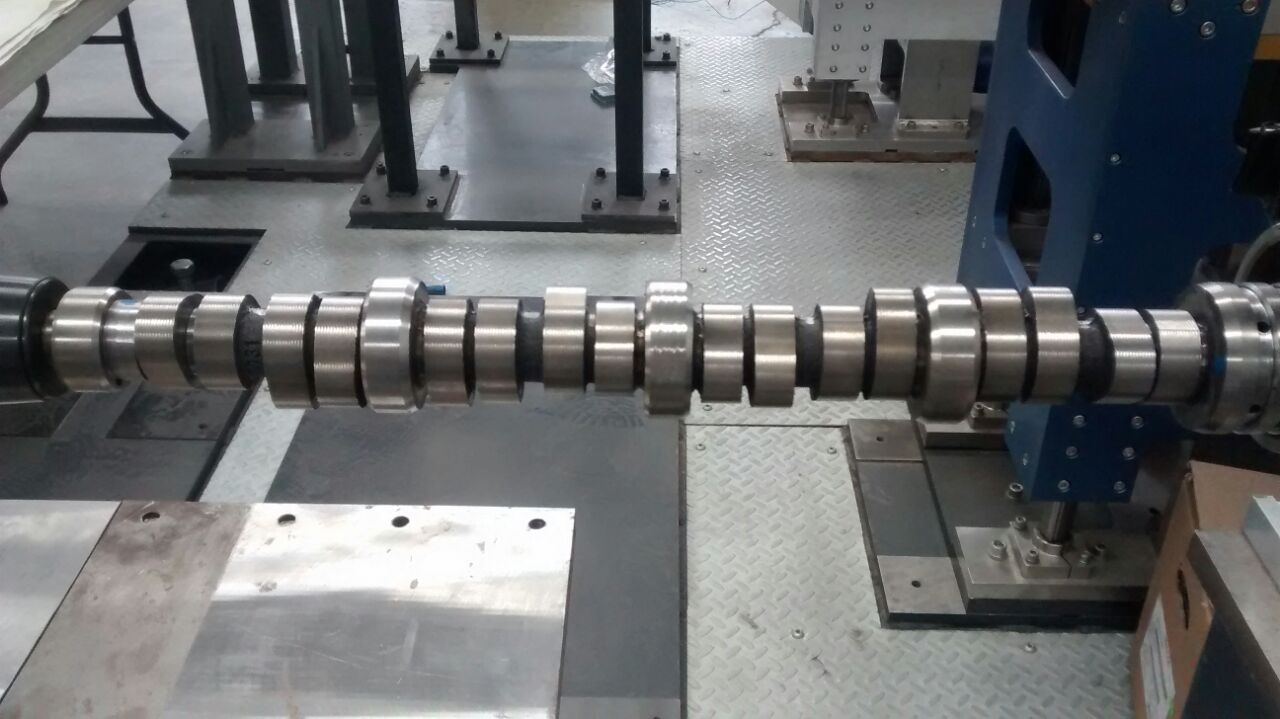
\includegraphics[width=\linewidth]{imagenes/view02.jpg}
\caption{Wide Picture}
\label{fig:view}
\end{figure*}

\begin{equation}
\cos^3 \theta =\frac{1}{4}\cos\theta+\frac{3}{4}\cos 3\theta
\label{eq:refname2}
\end{equation}

\begin{figure}[ht]\centering
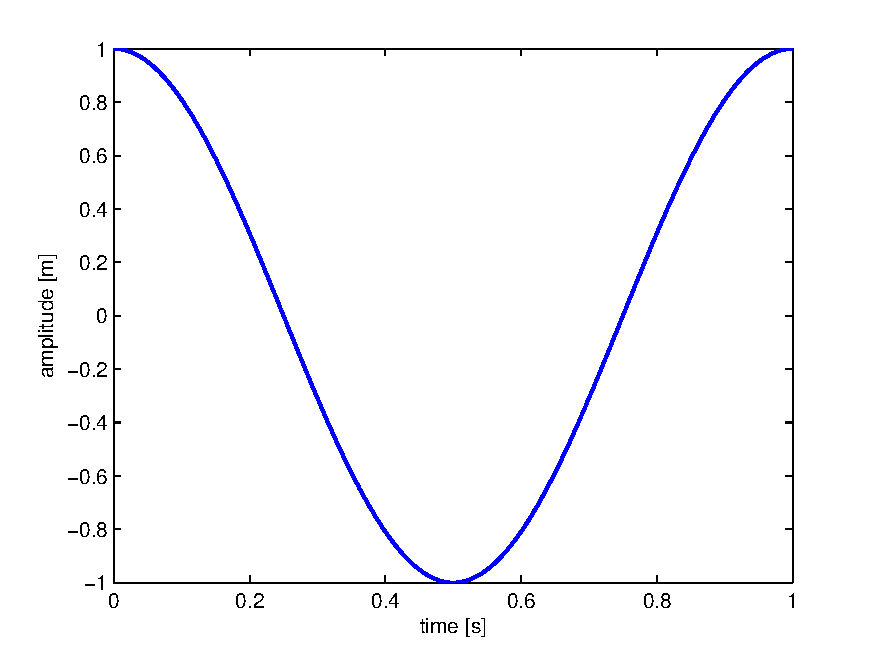
\includegraphics[width=\linewidth]{imagenes/results}
\caption{In-text Picture}
\label{fig:results}
\end{figure}

Reference to Figure \ref{fig:results}.

%------------------------------------------------

\section{Resultados}
Es la manera de presentar al lector los resultados obtenidos como producto de la investigación.

Puede ser de tres tipos:

\begin{enumerate}[noitemsep]
 \item Escrita: consiste en incorporar en forma de texto los datos estadísticos recopilados.
 \item Semitabular: se utiliza cuando se incorporan cifras a un texto y se tiene interés de hacerlas resaltar para facilitar su comparación.
 \item Tabular: consiste en presentar los datos numéricos de manera concreta, breve y ordenada a través de tablas y figuras con las especificaciones correspondientes. Se usa cuando se trata de muchos datos, cuando se desea indicar una relación que es difícil de explicar por escrito, o cuando se quiere facilitar la presentación de la información. Las figuras pueden ser fotografías, dibujos, mapas, diagramas de flujo, etc. La representación y análisis de los resultados debe ser completa, comprensible y precisa.
\end{enumerate}


\section{Discussion}
Compone el nuevo conocimiento que la investigación aporta a la ciencia; encontrándole un significado más amplio a las respuestas mediante su relación con otros conocimientos disponibles: leyes, teorías, etc.

\subsection{Sugerencias}

\begin{enumerate}[noitemsep]
 \item Describir cómo se llevaron a cabo las pruebas estadísticas, incluyendo las tablas que se utilizaron.
 \item Narrar organizadamente los resultados y no incluir solamente una serie de gráficas y tablas estadísticas.
 \item Analizar la relación existente entre el problema, los objetivos y las hipótesis planteadas al inicio de la investigación.
 \item Presentar los resultados obtenidos en la investigación, manifestando sus posibles explicaciones.
\end{enumerate}


\section{Conclusiones}
Es la interpretación de los resultados a la luz de un modelo teórico, haciendo una comparación con éste y precisando en qué medida dicho modelo puede considerarse confirmado o no.

\subsection{Sugerencias}

\begin{enumerate}[noitemsep]
 \item Deben hacer referencia directa a los problemas, objetivos e hipótesis de la investigación.
 \item Los problemas, objetivos e hipótesis se agruparán, ordenándolas según su orden de importancia, resumiendo los principales hallazgos y el significado de los datos obtenidos.
 \item Analizar cada uno de los objetivos propuestos para constatar si se lograron o no.
 \item Aceptar o rechazar cada una de  las hipótesis, si es que se plantearon.
 \item Aceptar de manera imparcial, los resultados obtenidos, aún cuando sean opuestos a lo que se deseaba.
 \item Elaborar comentarios acerca de cada una de las conclusiones.
 \item Demostrar y fundamentar los argumentos propuestos para el tratamiento o resolución del problema.
\end{enumerate}


\section*{Nomenclatura}
\noindent 
\begin{center}
\begin{tabular}{lp{6cm}}
$\Re$ & Campo de los números reales\\
$\mathbb{Z}$ & Campo de los números enteros\\
$D$ & Matriz de distancias \\
$d_{ii}$ & Distancia entre dos soluciones técnicas\\
$F$ & Conjunto de funciones\\
$f_i$ & Función\\
$CN$ & Conjunto de necesidades del cliente\\
$P$ & Plataforma\\
$p_i$ & Productos\\
$\Gamma$ & Componentes teóricos\\
$C$ & Conjunto de componentes\\
$c_{i}^{k}$ & Componentes\\
$ST$ & Conjunto de soluciones técnicas\\
SKU & \textit{Stock-keeping unit}\\
QFD & \textit{Quality function deployment}\\
$CN_{rod}$ & Necesidades de los rodados\\
$ST_{rod}$ & Soluciones técnicas de los rodados\\
$PP_{rod}$ & Propiedades de los rodados\\
$T_{CNPP}$ & Transformación de necesidades a propiedades\\
$T_{rdist}$ & Transformación de las distancias de los rodados
\end{tabular}
\end{center}

%------------------------------------------------
\phantomsection
\section*{Agradecimientos} % The \section*{} command stops section numbering
\addcontentsline{toc}{section}{Agradecimientos} % Adds this section to the table of contents

Es la parte donde se hace constar el nombre de todas las personas que han contribuido al desarrollo de la investigación  y a las instituciones que lo han apoyado. Es posible incluir en este apartado a familiares y amigos.

\begin{enumerate}[noitemsep]
 \item Deben ser sobrias y mesuradas.
 \item No elaborar dedicatorias de índole religiosa.
\end{enumerate}

%----------------------------------------------------------------------------------------
%	REFERENCE LIST
%----------------------------------------------------------------------------------------
\phantomsection
\bibliographystyle{unsrt}
\bibliography{sample,Bibliografia_BibTex.bib}

\begin{center}
\begin{tabular}{m{4cm} m{4cm}}

\includegraphics{foto_autor/homero_simpson.jpg} & \textbf{Homero Jay Simpson} Homero se cría en la granja de sus padres, Abraham y Mona Simpson. A mediados de los años 60, mientras Homero tiene entre nueve y doce años de edad. Homero asistió a la Escuela Secundaria de Springfield y en 1974, su último año, se enamora (por segunda vez) de Marge Bouvier. \\

\includegraphics{foto_autor/borola-burron2.png} & \textbf{Borola Tacuche} Nació en el seno de una muy rica y reconocida familia de la Ciudad de México. Alega haber sido una gran vedette de los teatros, razonamiento que le permite no limitarse y explorar oficios tan diversos como piloto de carreras, luchadora enmascarada, médico cirujano o ingeniera empírica.
\end{tabular}
\end{center}
%----------------------------------------------------------------------------------------

\end{document}
